\documentclass[12pt]{article}
\usepackage[utf8]{inputenc}
\usepackage{float}
\usepackage{amsmath}
\usepackage{amssymb}
\usepackage{multicol}
\usepackage[shortlabels]{enumitem}


\usepackage[hmargin=3cm,vmargin=6.0cm]{geometry}
%\topmargin=0cm
\topmargin=-2cm
\addtolength{\textheight}{6.5cm}
\addtolength{\textwidth}{2.0cm}
%\setlength{\leftmargin}{-5cm}
\setlength{\oddsidemargin}{0.0cm}
\setlength{\evensidemargin}{0.0cm}

%misc libraries goes here
\usepackage{tikz}

\begin{document}

\section*{Student Information }
%Write your full name and id number between the colon and newline
%Put one empty space character after colon and before newline
Full Name : Berk Ulutaş \\
Id Number :  2522084 \\

% Write your answers below the section tags
\section*{Answer 1}
\subsection*{1)} 
$M = (K,\Sigma, \Gamma, \Delta,s, F)$ \\
$K = \{s,p,q,r,f\}$ \\ 
$\Sigma = \{a,b\}$ \\ 
$\Gamma = \{a,b, \bot \}$ ($\bot$ to mark bottom of the stack)\\ 
$F = \{f\}$
\begin{equation*}
    \begin{split}
        \Delta = \{&((s,e,e),(p,\bot)),\\
                   &((p,a,e),(p,e)),\\
                   &((p,b,e),(p,e)),\\
                   &((p,e,e),(q,e)),\\
                   &((q,a,e),(q,a)),\\
                   &((q,b,e),(q,b)),\\
                   &((q,e,e),(r,e)),\\
                   &((r,a,e),(r,e)),\\
                   &((r,b,e),(r,e)),\\
                   &((r,\#,e),(t,e)),\\
                   &((t,a,a),(t,e)),\\
                   &((t,b,b),(t,e)),\\
                   &((t,e,\bot),(f,e)) \}
    \end{split}
\end{equation*}


\begin{center}
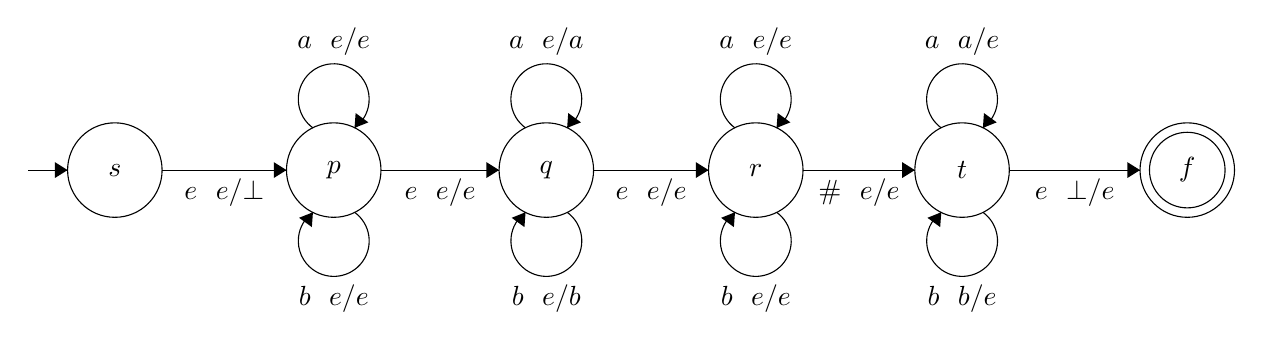
\begin{tikzpicture}[scale=0.2]
\tikzstyle{every node}+=[inner sep=0pt]
\draw [black] (6.7,-28.6) circle (3);
\draw (6.7,-28.6) node {$s$};
\draw [black] (20.6,-28.6) circle (3);
\draw (20.6,-28.6) node {$p$};
\draw [black] (34.1,-28.6) circle (3);
\draw (34.1,-28.6) node {$q$};
\draw [black] (47.4,-28.6) circle (3);
\draw (47.4,-28.6) node {$r$};
\draw [black] (60.5,-28.6) circle (3);
\draw (60.5,-28.6) node {$t$};
\draw [black] (74.8,-28.6) circle (3);
\draw (74.8,-28.6) node {$f$};
\draw [black] (74.8,-28.6) circle (2.4);
\draw [black] (1.2,-28.6) -- (3.7,-28.6);
\fill [black] (3.7,-28.6) -- (2.9,-28.1) -- (2.9,-29.1);
\draw [black] (9.7,-28.6) -- (17.6,-28.6);
\fill [black] (17.6,-28.6) -- (16.8,-28.1) -- (16.8,-29.1);
\draw (13.65,-29.1) node [below] {$e\mbox{ }\mbox{ }e/\bot$};
\draw [black] (19.277,-25.92) arc (234:-54:2.25);
\draw (20.6,-21.35) node [above] {$a\mbox{ }\mbox{ }e/e$};
\fill [black] (21.92,-25.92) -- (22.8,-25.57) -- (21.99,-24.98);
\draw [black] (21.923,-31.28) arc (54:-234:2.25);
\draw (20.6,-35.85) node [below] {$b\mbox{ }\mbox{ }e/e$};
\fill [black] (19.28,-31.28) -- (18.4,-31.63) -- (19.21,-32.22);
\draw [black] (23.6,-28.6) -- (31.1,-28.6);
\fill [black] (31.1,-28.6) -- (30.3,-28.1) -- (30.3,-29.1);
\draw (27.35,-29.1) node [below] {$e\mbox{ }\mbox{ }e/e$};
\draw [black] (32.777,-25.92) arc (234:-54:2.25);
\draw (34.1,-21.35) node [above] {$a\mbox{ }\mbox{ }e/a$};
\fill [black] (35.42,-25.92) -- (36.3,-25.57) -- (35.49,-24.98);
\draw [black] (35.423,-31.28) arc (54:-234:2.25);
\draw (34.1,-35.85) node [below] {$b\mbox{ }\mbox{ }e/b$};
\fill [black] (32.78,-31.28) -- (31.9,-31.63) -- (32.71,-32.22);
\draw [black] (37.1,-28.6) -- (44.4,-28.6);
\fill [black] (44.4,-28.6) -- (43.6,-28.1) -- (43.6,-29.1);
\draw (40.75,-29.1) node [below] {$e\mbox{ }\mbox{ }e/e$};
\draw [black] (46.077,-25.92) arc (234:-54:2.25);
\draw (47.4,-21.35) node [above] {$a\mbox{ }\mbox{ }e/e$};
\fill [black] (48.72,-25.92) -- (49.6,-25.57) -- (48.79,-24.98);
\draw [black] (48.723,-31.28) arc (54:-234:2.25);
\draw (47.4,-35.85) node [below] {$b\mbox{ }\mbox{ }e/e$};
\fill [black] (46.08,-31.28) -- (45.2,-31.63) -- (46.01,-32.22);
\draw [black] (50.4,-28.6) -- (57.5,-28.6);
\fill [black] (57.5,-28.6) -- (56.7,-28.1) -- (56.7,-29.1);
\draw (53.95,-29.1) node [below] {$\#\mbox{ }\mbox{ }e/e$};
\draw [black] (63.5,-28.6) -- (71.8,-28.6);
\fill [black] (71.8,-28.6) -- (71,-28.1) -- (71,-29.1);
\draw (67.65,-29.1) node [below] {$e\mbox{ }\mbox{ }\bot/e$};
\draw [black] (59.177,-25.92) arc (234:-54:2.25);
\draw (60.5,-21.35) node [above] {$a\mbox{ }\mbox{ }a/e$};
\fill [black] (61.82,-25.92) -- (62.7,-25.57) -- (61.89,-24.98);
\draw [black] (61.823,-31.28) arc (54:-234:2.25);
\draw (60.5,-35.85) node [below] {$b\mbox{ }\mbox{ }b/e$};
\fill [black] (59.18,-31.28) -- (58.3,-31.63) -- (59.11,-32.22);
\end{tikzpicture}
\end{center}
\subsection*{2)}
$M = (K,\Sigma, \Gamma, \Delta, s, F)$ \\
$K = \{s,p,q,r,t,f\}$ \\ 
$\Sigma = \{a,b\}$ \\ 
$\Gamma = \{a,b, \bot \}$ ($\bot$ to mark bottom of the stack)\\ 
$F = \{f\}$
\begin{equation*}
    \begin{split}
        \Delta = \{&((s,e,e),(p,\bot)),\\
                   &((p,c,e),(p,c)),\\
                   &((p,e,e),(q,e)),\\
                   &((q,a,e),(q,a)),\\
                   &((q,b,e),(q,b)),\\
                   &((q,e,e),(r,e)),\\
                   &((r,a,a),(r,e)),\\
                   &((r,b,b),(r,e)),\\
                   &((r,e,e),(t,e)),\\
                   &((t,c,c),(t,e)),\\
                   &((t,e,\bot),(f,e)) \}
    \end{split}
\end{equation*}

\begin{center}
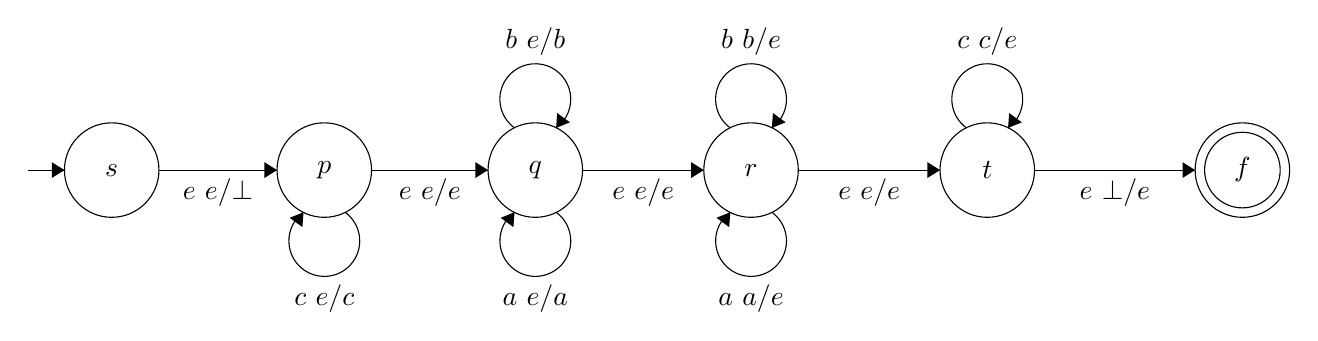
\begin{tikzpicture}[scale=0.2]
\tikzstyle{every node}+=[inner sep=0pt]
\draw [black] (5.1,-9.1) circle (3);
\draw (5.1,-9.1) node {$s$};
\draw [black] (18.6,-9.1) circle (3);
\draw (18.6,-9.1) node {$p$};
\draw [black] (32,-9.1) circle (3);
\draw (32,-9.1) node {$q$};
\draw [black] (45.7,-9.1) circle (3);
\draw (45.7,-9.1) node {$r$};
\draw [black] (60.7,-9.1) circle (3);
\draw (60.7,-9.1) node {$t$};
\draw [black] (76.9,-9.1) circle (3);
\draw (76.9,-9.1) node {$f$};
\draw [black] (76.9,-9.1) circle (2.4);
\draw [black] (8.1,-9.1) -- (15.6,-9.1);
\fill [black] (15.6,-9.1) -- (14.8,-8.6) -- (14.8,-9.6);
\draw (11.85,-9.6) node [below] {$e\mbox{ }e/\bot$};
\draw [black] (19.923,-11.78) arc (54:-234:2.25);
\draw (18.6,-16.35) node [below] {$c\mbox{ }e/c$};
\fill [black] (17.28,-11.78) -- (16.4,-12.13) -- (17.21,-12.72);
\draw [black] (-0.2,-9.1) -- (2.1,-9.1);
\fill [black] (2.1,-9.1) -- (1.3,-8.6) -- (1.3,-9.6);
\draw [black] (21.6,-9.1) -- (29,-9.1);
\fill [black] (29,-9.1) -- (28.2,-8.6) -- (28.2,-9.6);
\draw (25.3,-9.6) node [below] {$e\mbox{ }e/e$};
\draw [black] (33.323,-11.78) arc (54:-234:2.25);
\draw (32,-16.35) node [below] {$a\mbox{ }e/a$};
\fill [black] (30.68,-11.78) -- (29.8,-12.13) -- (30.61,-12.72);
\draw [black] (35,-9.1) -- (42.7,-9.1);
\fill [black] (42.7,-9.1) -- (41.9,-8.6) -- (41.9,-9.6);
\draw (38.85,-9.6) node [below] {$e\mbox{ }e/e$};
\draw [black] (48.7,-9.1) -- (57.7,-9.1);
\fill [black] (57.7,-9.1) -- (56.9,-8.6) -- (56.9,-9.6);
\draw (53.2,-9.6) node [below] {$e\mbox{ }e/e$};
\draw [black] (63.7,-9.1) -- (73.9,-9.1);
\fill [black] (73.9,-9.1) -- (73.1,-8.6) -- (73.1,-9.6);
\draw (68.8,-9.6) node [below] {$e\mbox{ }\bot/e$};
\draw [black] (44.377,-6.42) arc (234:-54:2.25);
\draw (45.7,-1.85) node [above] {$b\mbox{ }b/e$};
\fill [black] (47.02,-6.42) -- (47.9,-6.07) -- (47.09,-5.48);
\draw [black] (59.377,-6.42) arc (234:-54:2.25);
\draw (60.7,-1.85) node [above] {$c\mbox{ }c/e$};
\fill [black] (62.02,-6.42) -- (62.9,-6.07) -- (62.09,-5.48);
\draw [black] (30.677,-6.42) arc (234:-54:2.25);
\draw (32,-1.85) node [above] {$b\mbox{ }e/b$};
\fill [black] (33.32,-6.42) -- (34.2,-6.07) -- (33.39,-5.48);
\draw [black] (47.023,-11.78) arc (54:-234:2.25);
\draw (45.7,-16.35) node [below] {$a\mbox{ }a/e$};
\fill [black] (44.38,-11.78) -- (43.5,-12.13) -- (44.31,-12.72);
\end{tikzpicture}
\end{center}

\section*{Answer 2}
Let $G=(V, \Sigma, R, S)$ where \\
$V = \{S, 0, 1\}$ \\ 
$\Sigma = \{0,1\}$ \\ 
$R = {S \rightarrow 0S0 \mbox{ }|\mbox{ } 1 }$ \\

This context-free grammar G, generates Context-free language $L = L(G) = \{0^n10^n \mbox{ }| \mbox{ } n \geq 0 \}$. It generates strings: 
$$1, 010, 00100 \dots$$. 

Add rule $S \rightarrow SS$ to grammar and $R$ becomes: 
$$R = S \rightarrow SS \mbox{ } | \mbox{ } 0S0 \mbox{ } | \mbox{ } 1  $$

It is clear that with the newly added rule, this grammar cannot produce empty string($e$). However, $L^*$ includes empty string(e). Thus, adding rule $S \rightarrow SS $ does not produce $L^*$
\section*{Answer 3}
\subsection*{1)}
\begin{itemize}
    \item Let x will be our stack symbol
    \item $L_1 = \{a^nb^n | n \geq 0\}$. $L_1$ is an S-CFL. We can construct an S-PDA which recognizes $L_1$. For each "a" read from the input, push "x" onto the stack. When machine starts reading b's, pop "x" for every "b" read. If the input is completely read and the stack is empty, the S-PDA accepts input string. This S-PDA works since, b's come after a's. First we count number of a's then during popping we check number of b's is equal to number of a's. 
    \item $L_2 = \{w | w \in \{a,b\}^* \mbox{ and the number of a's in w is not equal to number of b's in w}\}$. $L_2$ is not an S-CFL. Think normal PDA for this question. It keeps difference between the number of a's and number of b's with which one is more. If stack has a's on it this means in currrent situation a's more than b's or vice versa. Since S-PDA has only one stack symbol it cannot differentiate between a's and b's when counting them on the stack. Thus, it cannot determine if the number of a's is different from the number of b's in the input string. 
    \item $L_3 = \{a^nb^{n+m}c^m | m,n  \in \mathbb{N}\}$ $L_3$ is an S-CFL. We can construct S-PDA which recognizes $L_3$. Think $L_3$ like this $\{a^nb^nb^mc^m | m,n \in \mathbb{N}\}$. For each "a" read from the input push "x" onto the stack. When machine starts reading b's, pop "x" from stack for each b read(these are the 'n' number of b's). When stack becomes empty push "x" onto stack for each b read (these are the 'm' number of b's). When it starts reading c's. pop "x" from stack for each c read. If the input is completely read and the stack is empty, the S-PDA accepts input string. This S-PDA works since, c's comes after b's and b's comes after a's. First we count number of a's(n) with pushing x onto the stack, then we process n b's with popping x from stack. After that we need to determine m. So, we count b's(m) with stack. Then we check is there m c's. 
\end{itemize}

\subsection*{2)}
$L_4  = \{a^nb^{2n} | n \geq 0 \}$ $L_4$ is an S-CFL. We can construct an S-PDA which recognizes $L_4$. For each "a" read from the input, push two "x" onto the stack. When machine starts reading b's, pop "x" for every "b" read. If the input is completely read and the stack is empty, the S-PDA accepts input string. \\
$G = \{V, \Sigma, R, S\}$ where
\begin{itemize}
    \item $V = {S,a,b}$
    \item $\Sigma = {a,b}$
    \item $R = {S \rightarrow aSbb \mbox{ }| \mbox{ }  e}$
\end{itemize}



\subsection*{3)}
The minimal memory element that must be added to finite automata to recognize S-CFLs is a \textbf{Counter}.

\subsection*{4)}
\begin{itemize}
    \item Function of counter to keep track of a single integer value. It can be incremented or decremented by automaton during processing input. 
    \item The counter is less powerful than a stack since, it cannot keep multiple elements.
    \item By using counter, a finite automaton can recognize S-CFLs. Since, Stack with just one stack symbol basically a counter. It cannot keep multiple elements, just keeps a single integer value like a counter. We can mimic what stack(with single stack symbol) do with a counter, by increasing the counter instead of pushing the stack.
\end{itemize}

\subsection*{5)}
No it is not closed under complementation. Here is a counter example: 

\begin{itemize}
    \item Consider \\ $L_1 = \{a^nb^n | n \geq 0\}$ \\$L_2 = \{w | w \in \{a,b\}^* \mbox{ and the number of a's in w is not equal to number of b's in w}\}$. \\  
    from Question 3.1 
    \item The language $L_1 = \{a^nb^n | n \geq 0\}$ is a S-CFL as shown in Question 3.1.
    \item Now consider the complement of $L_1$, let's say $L_1'$. $$L_1' = \{w | w \in \{a,b\}^* \mbox{ and do not have the form $a^nb^n, n \geq 0$}\}$$
    \item In other words, $L_1'$ is also includes of strings where the number of a's is not equal to the number of b's (which is $L_2$). We have shown that $L_2$ is not a S-CFL. in Question 3.1. So, $L_1'$ is also not a S-CFL
    \item Let's take $"baababa"$ an example string from $L_1'$ which is also in $L_2$. 
    \item We cannot accept $"baababa"$ with a S-PDA. Since S-PDA has only one stack symbol it cannot differentiate between a’s and b’s when counting them on the stack. Thus, it cannot determine if the number of a’s is different from the number of b’s in the input string.
\end{itemize}



 

\end{document}


